% !TEX root = ../ClassicThesis_DEIB.tex

\chapter{Localization and navigation systems in GRAPE} \label{chap:localization}

The studies of \cite{outdoorNavigation}, that analyze main issues in autonomous mobile robot navigation, identify three main problems related to outdoor autonomous navigation:
\begin{itemize}
	\item the unstructured environment where the actions take place, in opposition to the clear and definite one that is typical in indoor navigation (flat floor, right angles, smooth surfaces)
	\item multiple sensors required, to be aware enough of the surrounding environment, in order to take decisions
	\item moving obstacles, like for example pedestrians or cars in a city road
\end{itemize}
The system developed in the context of \ac{GRAPE} project suffers critically mostly of the first two point listed above. Indeed, the vineyard environment, even if characterized by a high degree of regularity in the global structure, due to the presence of parallel rows of trees, presents strongly difficulties regarding lack of structure in the terrain configuration (steep, bumpy, clay-rich, muddy, according to the weather conditions and the intrinsic composition and morphology of the terrain) and in the obstacles (non-straight surfaces, different reflectivity and lighting conditions). The problem of the fusion of the data coming from the disparates sensors mounted on board of the robot was already addressed from a theoretically point of view in Section \ref{sec:sensorFusion}, and it's the major component in the localization system of the robot. Note that, being our robot an agricultural \ac{UGV}, the problem of moving obstacles is not particularly relevant, since they are most likely to be humans, aware of the robot presence and functionalities, or small wild animals (\textit{e.g.} foxes, hares, cats) in remote cases, that however have a very low probability of approaching the Husky base during movement.

\par In the next section we are going to analyze with detail the configuration of both the odometry and navigation systems running on the \ac{UGV}. It will be clear that both the problems, even if eventually solved using \textit{off-the-shelf} solutions, were all but simple problems and required a real understanding of the numerous problems that arose.

\section{Odometry system}\label{sec:odometrySystem}

The configuration of a robust odometry system for vineyard navigation has been a workpoint since the beginning of the project, because of the expected (and actual) strong instability of the wheel odometry. To the reasons mentioned at the beginning of the Chapter, we recall also the intrinsic lack of precision due to skid steering kinematics of the Husky base.
We can describe the search for a robust odometry system for the \ac{UGV} in three main phases:
\begin{enumerate}
	\item As hinted in Section \ref{sec:sensorFusion}, in the early phases of \ac{GRAPE} project, the designated sensor fusion framework was \textbf{ROAMFREE}, that gave proof of good functioning in the past (see Section \ref{sec:sensorFusion} for precise references). ROAMFREE platform provides multi-sensors pose tracking and it is designed to be flexible and to adapt to every kind of mobile robotic platform. The tracking module is based on Gauss-Newton minimization of the error functions associated to sensor readings. In order to improve generality, physical sensors are abstracted with \textit{logical sensors}, which are characterized only by the type of the proprioceptive measurement they produce. Another ROAMFREE module provides instead self-calibration modules, using error models for each sensor category to provide on-line correction of common sources of distortion, bias and noise (\textit{e.g.} hard and soft magnetic distortion, sensor displacement or misalignment). The usage of ROAMFREE framework was specified in the project proposal, thus it was of course the default choice for the sensor fusion framework in the first \textit{integration week} in Garriguella (ES), before the beginning of this thesis work. The \ac{ROS} implementation of ROAMFREE is still experimental, anyhow a configuration was identified to fit the requirements. Unfortunately, the same configuration turned out to perform poorly during the second integration week in Casciana Terme (IT). This was caused by concurrence of:
	\begin{itemize}
		\item presence of a significant slope in the vineyard, in opposition to the flat (even if bumpy) terrain in Garriguella
		\item difficulty to handle inaccurate configuration of magnetometer and \ac{IMU}
		\item overall trickiness in the configuration procedure, being ROAMFREE integration with \ac{ROS} still experimental
	\end{itemize}
	The low performances of this framework in this context were pretty clear, so we opted for a more tested and consolidated solution, \textbf{Robot Localization}.
	
	\item The configuration of Robot Localization requires, for each fused sensor, a configuration vector, in which specify which components of the input estimate should be fused into the final pose estimate. Note that the the configuration vector is given in the \textit{frame\_id} of the input message: for example, consider a velocity sensor that produces a \textit{geometry\_msgs/TwistWithCovarianceStamped} message with a \textit{frame\_id} of \textit{velocity\_sensor\_frame}. We now assume that the transform would convert $X$ velocity in the \\ \textit{velocity\_sensor\_frame} to $Z$ velocity in the \textit{base\_link\_frame}. To include the $\dot{X}$ data from the sensor into the filter, the configuration vector should set the $\dot{X}$ velocity value to true, and not the $\dot{Z}$ velocity value. 
\par In table \ref{tab:robotLocalizationConfig} you can see the configuration vectors for the sensors taken as input from Robot Localization. Note that, for example, GPS only gives a contribute about $x$ and $y$, since the altitude estimation of GPS is often not precise, and it provides no information about the robot orientation. Our configuration of Robot Localization relies on \textbf{two} different \ac{EKF} nodes in cascade:
	\begin{itemize}
		\item a \textit{local} localization node, that fuses continuous data, and estimates the position and orientation of the \textit{base\_link} frame of the robot inside the \textit{odom} frame \textit{i.e.} the frame fixed in the initial position of the robot. In other words, the task of the node is to publish \textit{odom} $\rightarrow$ \textit{base\_link tf} transform (see Section \ref{sec:tf} for recall). 
		\item a \textit{global} localization node, that also fuses low frequency sensors \textit{i.e.} GPS, and estimates the position and orientation of \textit{odom} frame inside \textit{map} frame. The \textit{map} $\rightarrow$ \textit{odom} trasfomation "adjusts" the position of frame \textit{odom} in order to contextualize the position of the \ac{UGV} inside the map. Otherwise, the robot pose would be tracked only with respect to its initial position (origin of \textit{odom} frame), but no positioning inside a map would be provided.
 	\end{itemize}
In Figure \ref{fig:cascadeRobotLocalization} you can see the computation graph of the aforementioned odometry system: you can observe that:
	\begin{itemize}
		\item both nodes write on \textit{tf} topic the respective \textit{tf} transforms
		\item the local node takes \ac{IMU} (\textit{/imu/data} topic) and wheels \\ (\textit{/husky\_velocity\_controller/odom} topic) estimate for the fusion task
		\item the global node takes as input the pose estimate from GPS (\textit{/odometry\_gps} topic), and the pose estimate from the local node (\textit{/odometry/ekf\_local\_filtered} topic), to implement the cascade scheme.
	\end{itemize}

	\item Even if the cascade produced a pretty precise odometry estimate, the odometry computation was shrunk in a single \ac{EKF} node for two main reasons:
	\begin{itemize}
		\item as we'll describe in Section \ref{sec:navigationSystem}, the navigation system switched to a mapless configuration, so the \textit{tf} transform  \textit{map} $\rightarrow$ \textit{odom} became useless
		\item the \ac{EKF}s cascade configuration led to a short delay in the odometry computation (\textasciitilde200-300 ms). This caused some problems with the obstacles detection implemented through \ac{LIDAR} data, that were processed with negligible delay, and especially when the robot moved from the end of a row of vines to the beginning of another one. 
	\end{itemize}
\end{enumerate}

\setlength\tabcolsep{3pt}
\begin{table}[tb]
\footnotesize
\centering
\begin{tabularx}{0.85\textwidth}{X|XXXXXXXXXXXXXXXX}
\hline
\toprule
\tableheadline{l}{ }  &
\tableheadline{r}{$x$}  &
\tableheadline{r}{$y$}  &
\tableheadline{r}{$z$}  &
\tableheadline{r}{$\psi$}  	&
\tableheadline{r}{$\theta$}  	&
\tableheadline{r}{$\phi$}	&
\tableheadline{r}{$\dot{x}$}  	&
\tableheadline{r}{$\dot{y}$}  		&
\tableheadline{r}{$\dot{z}$}   	&
\tableheadline{r}{$\dot{\psi}$}   		&
\tableheadline{r}{$\dot{\theta}$}	&
\tableheadline{r}{$\dot{\phi}$}   		&
\tableheadline{r}{$\dot{\theta}$}   	&
\tableheadline{r}{$\ddot{x}$}   		&
\tableheadline{r}{$\ddot{y}$}  		 &
\tableheadline{r}{$\ddot{z}$}   		\\
\midrule
\tablefirstcol{l}{Wheels}
&  \ding{51} & \ding{51}  & \ding{51} &  &  & \ding{51} &\ding{51}  &\ding{51}  &\ding{51}  &  &  &  &  &  &  & \\
\midrule
\tablefirstcol{l}{IMU}
&  &   & & \ding{51} &  \ding{51} &  \ding{51}&  &  & &  & \ding{51} &\ding{51}  & \ding{51} & \ding{51} &  & \\
\midrule
\tablefirstcol{l}{GPS points}
&  \ding{51}& \ding{51}  &  &  &  &  &  &  &  &  &  &  &  &  &  & \\
\bottomrule
\end{tabularx}
\caption[Robot localization configuration]{\textit{Configuration vectors for the sensors fused for odometry estimation, using Robot Localization.}}
\label{tab:robotLocalizationConfig}
\end{table}
\setlength\tabcolsep{6pt}

\begin{figure}
	\centering
	\subfloat[]{%
		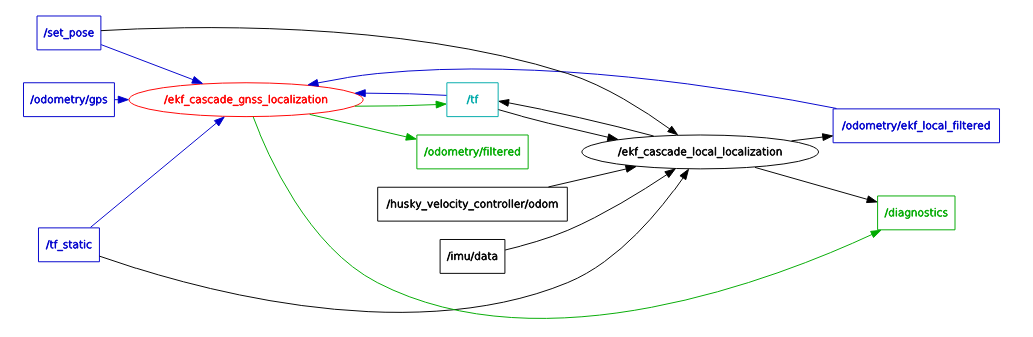
\includegraphics[width=0.9\textwidth]{Images/localization/cascadeGNSSgraph.png}
		\label{fig:cascadeGNSSgraph}} \\
	\subfloat[]{%
		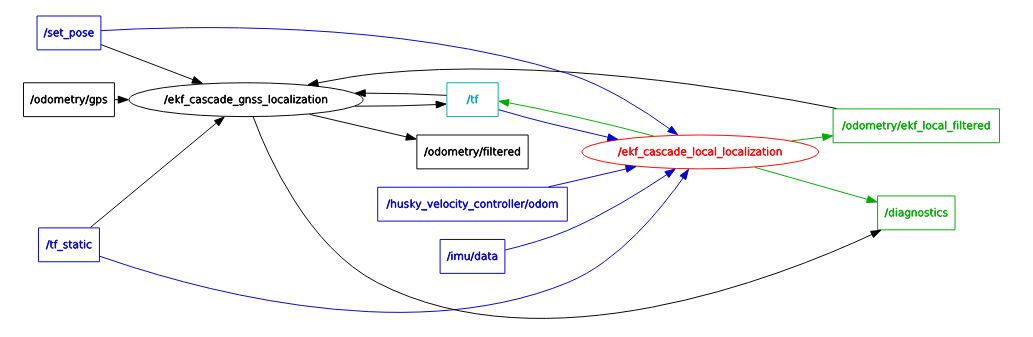
\includegraphics[width=0.9\textwidth]{Images/localization/cascadeLocalGraph.png}
		\label{fig:cascadeLocalGraph}}
	\caption{\textit{Computation graph of the cascade of Robot Localization nodes; in blue, the input topics, and in green the output topics, of the nodes highlighted in red.}}
	\label{fig:cascadeRobotLocalization}
\end{figure}


\section{Navigation system}\label{sec:navigationSystem}

We already anticipated in Section \ref{sec:navigationStack} that the reference navigation framework is \textbf{Move Base}, that is an \textit{off-the-shelf} \ac{ROS} software stack for autonomous navigation (see Figure \ref{fig:navStack} for a graphical representation of the main software modules of Move Base). Since, as already stated, this framework usually provides very stable autonomous navigation in indoor mapped environment, the first attempt was to shift the same configuration in the vineyard environment. 
In this Section we'll explain the steps from this initial naive solution to the final accepted one.

\subsection{Navigation in mapped environment with AMCL}

Before the robot could be able to navigate the vineyard, the navigation in mapping environment required a preparatory \textit{mapping} phase; in particular, this is a \ac{SLAM} problem, that is the computational problem of constructing or updating a map of an unknown environment, while simultaneously keeping track of an agent's (the \ac{UGV}) location within it. Note that \textit{localization} is a different task with respect to \textit{odometry estimate}, because the first aims to estimate the position of the robot inside a map, while the latter aims to estimate the position of the robot with respect to its initial pose. More technically, in the \ac{ROS} framework \textit{odometry estimate} algorithms publish the \textit{tf} transform from \textit{odom} frame to \textit{base\_link} frame, while \textit{localization} algorithms publish the one from \textit{map} to \textit{odom}.

\par Even if \ac{SLAM} is a \textit{chicken-and-egg} problem (localization would be easy in a known map, under some assumptions, and mapping would be easy if the robot position is assumed known), several algorithms exist that solve, even if approximately, the \ac{SLAM} problem. In the early phases of \ac{GRAPE}, previous to this thesis work and described in \cite{grapeAltroPaper}, three different \ac{SLAM} algorithms were tested in our specific environment: \textit{Gmapping}, \textit{Google's Cartographer} and \textit{KartoSLAM}, and \textbf{Gmapping} algorithm was selected because of its performance and efficiency in terms of computational load. In Figure \ref{fig:vineyardMap} you can see the map created in Mas Llunes during the last integration week, using Gmapping. The accomplished accuracy of the maps was satisfying, but actually a lot of problems occurred in the main phase, that is the autonomous navigation of the robot in the mapped environment. The most relevant problems that emerged were the following ones. 

\begin{description}
\item[AMCL in the vineyard map] \hfill \\
As you can see in Figure \ref{fig:navStack}, an optional node called \textbf{amcl} exists, that provides a \ac{ROS} implementation of \ac{AMCL} algorithm \parencite{amcl}. \ac{AMCL} is a localization algorithm, that uses a particle filter to provide a \textit{belief} \textit{i.e.} the robot's estimate of its current state, through a probability density function distributed over the state space. A single particle represents an hypothesis about the real pose of the robot in the environment (see Figure \ref{fig:amclAlgoritmo}); thus, regions in the state space with many particles correspond to a greater probability that the robot will be there, and regions with few particles are unlikely to be where the robot is.

\par In \ac{AMCL} each particle is assigned a weight that correspond to the probability that, had the robot been at the state of the particle, it would perceive what its sensors have actually sensed (in particular, \textit{amcl} \ac{ROS} package is only capable to deal with laser scans as sensor input); this weight is used in the algorithm to select the particles that are going to survive through iterations. For this reason, the algorithm requires both a sensor model of the used sensors, and a motion model of the involved robot, in order to update the \textit{belief}. In Figure \ref{fig:motionModelExample} you can see several steps of \textit{belief} update, only based on the motion model of the robot. Pseudo code of Monte Carlo Localization is provided in Algorithm \ref{alg:mcl}.

\begin{algorithm}
\caption{Monte Carlo Localization($X_{t-1},u_t,z_t$)}\label{alg:mcl}
\begin{algorithmic}[1]
\State $X_t=\emptyset$ 				\Comment{$X_t$ is belief about the robot state}
\State $\overline{X}_t=\emptyset$
\State for $m=1$ to $M$: 				\Comment{$M$ is number of particles}
\Indent
	\State $x^{[m]}_t=$ motion\_update($u_t,x^{[m]}_{t-1}$)	 \Comment{$u_z$ is actuation command}
	\State $w^{[m]}_t=$ sensor\_update($z_t,x^{[m]}_{t}$)	\Comment{$z_t$ are sensed data}
	\State $\overline{X}_t = {X}_t + \big \langle x^{[m]}_t, w^{[m]}_t \big \rangle$
\EndIndent
\State endfor
\State for $m=1$ to $M$: 
\Indent
	\State draw $x^{[m]}_t$ from $\overline{X}_t$ with probability $\propto w^{[m]}_t$
	\State $X_t=X_t+x^{[m]}_t$
\EndIndent
\State endfor
\State return $X_t$
\end{algorithmic}
\end{algorithm}

\begin{figure}
	\centering
	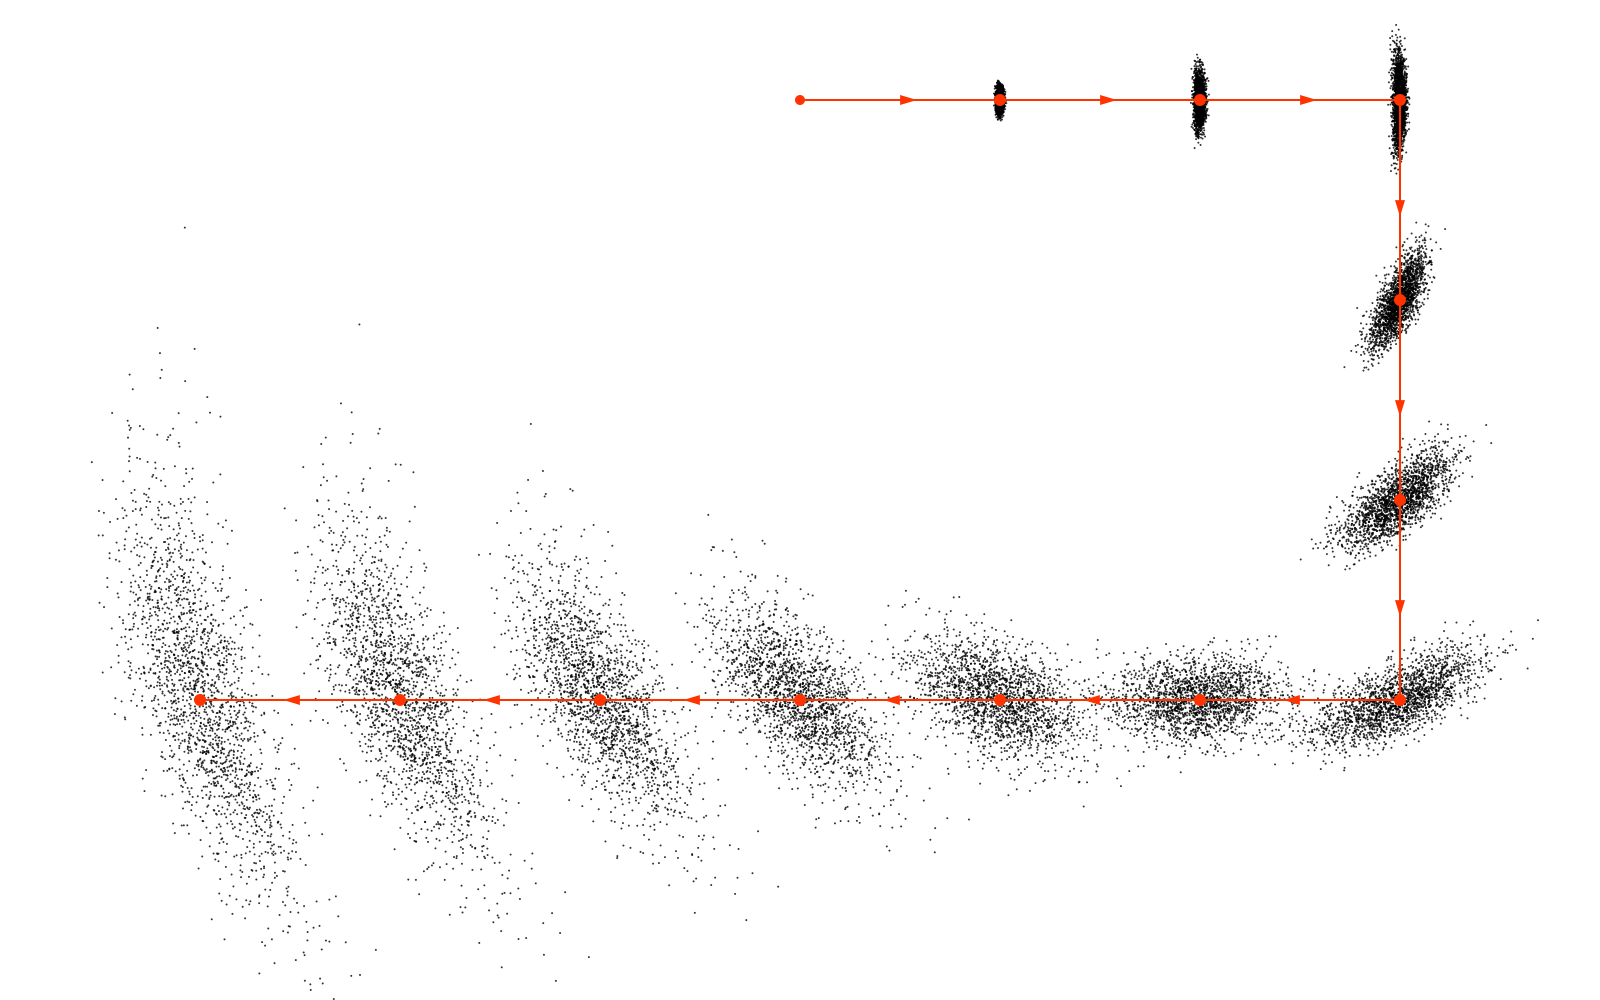
\includegraphics[width=0.8\textwidth]{Images/localization/motionModel.png}
	\caption{\textit{Evolution of the belief computed by \ac{AMCL}, taking into account the motion update only (ignoring the sensor update).}}
	\label{fig:motionModelExample}
\end{figure}


\begin{figure}
	\begin{minipage}[c]{.5\textwidth}
		\centering
		\subfloat[]{%
		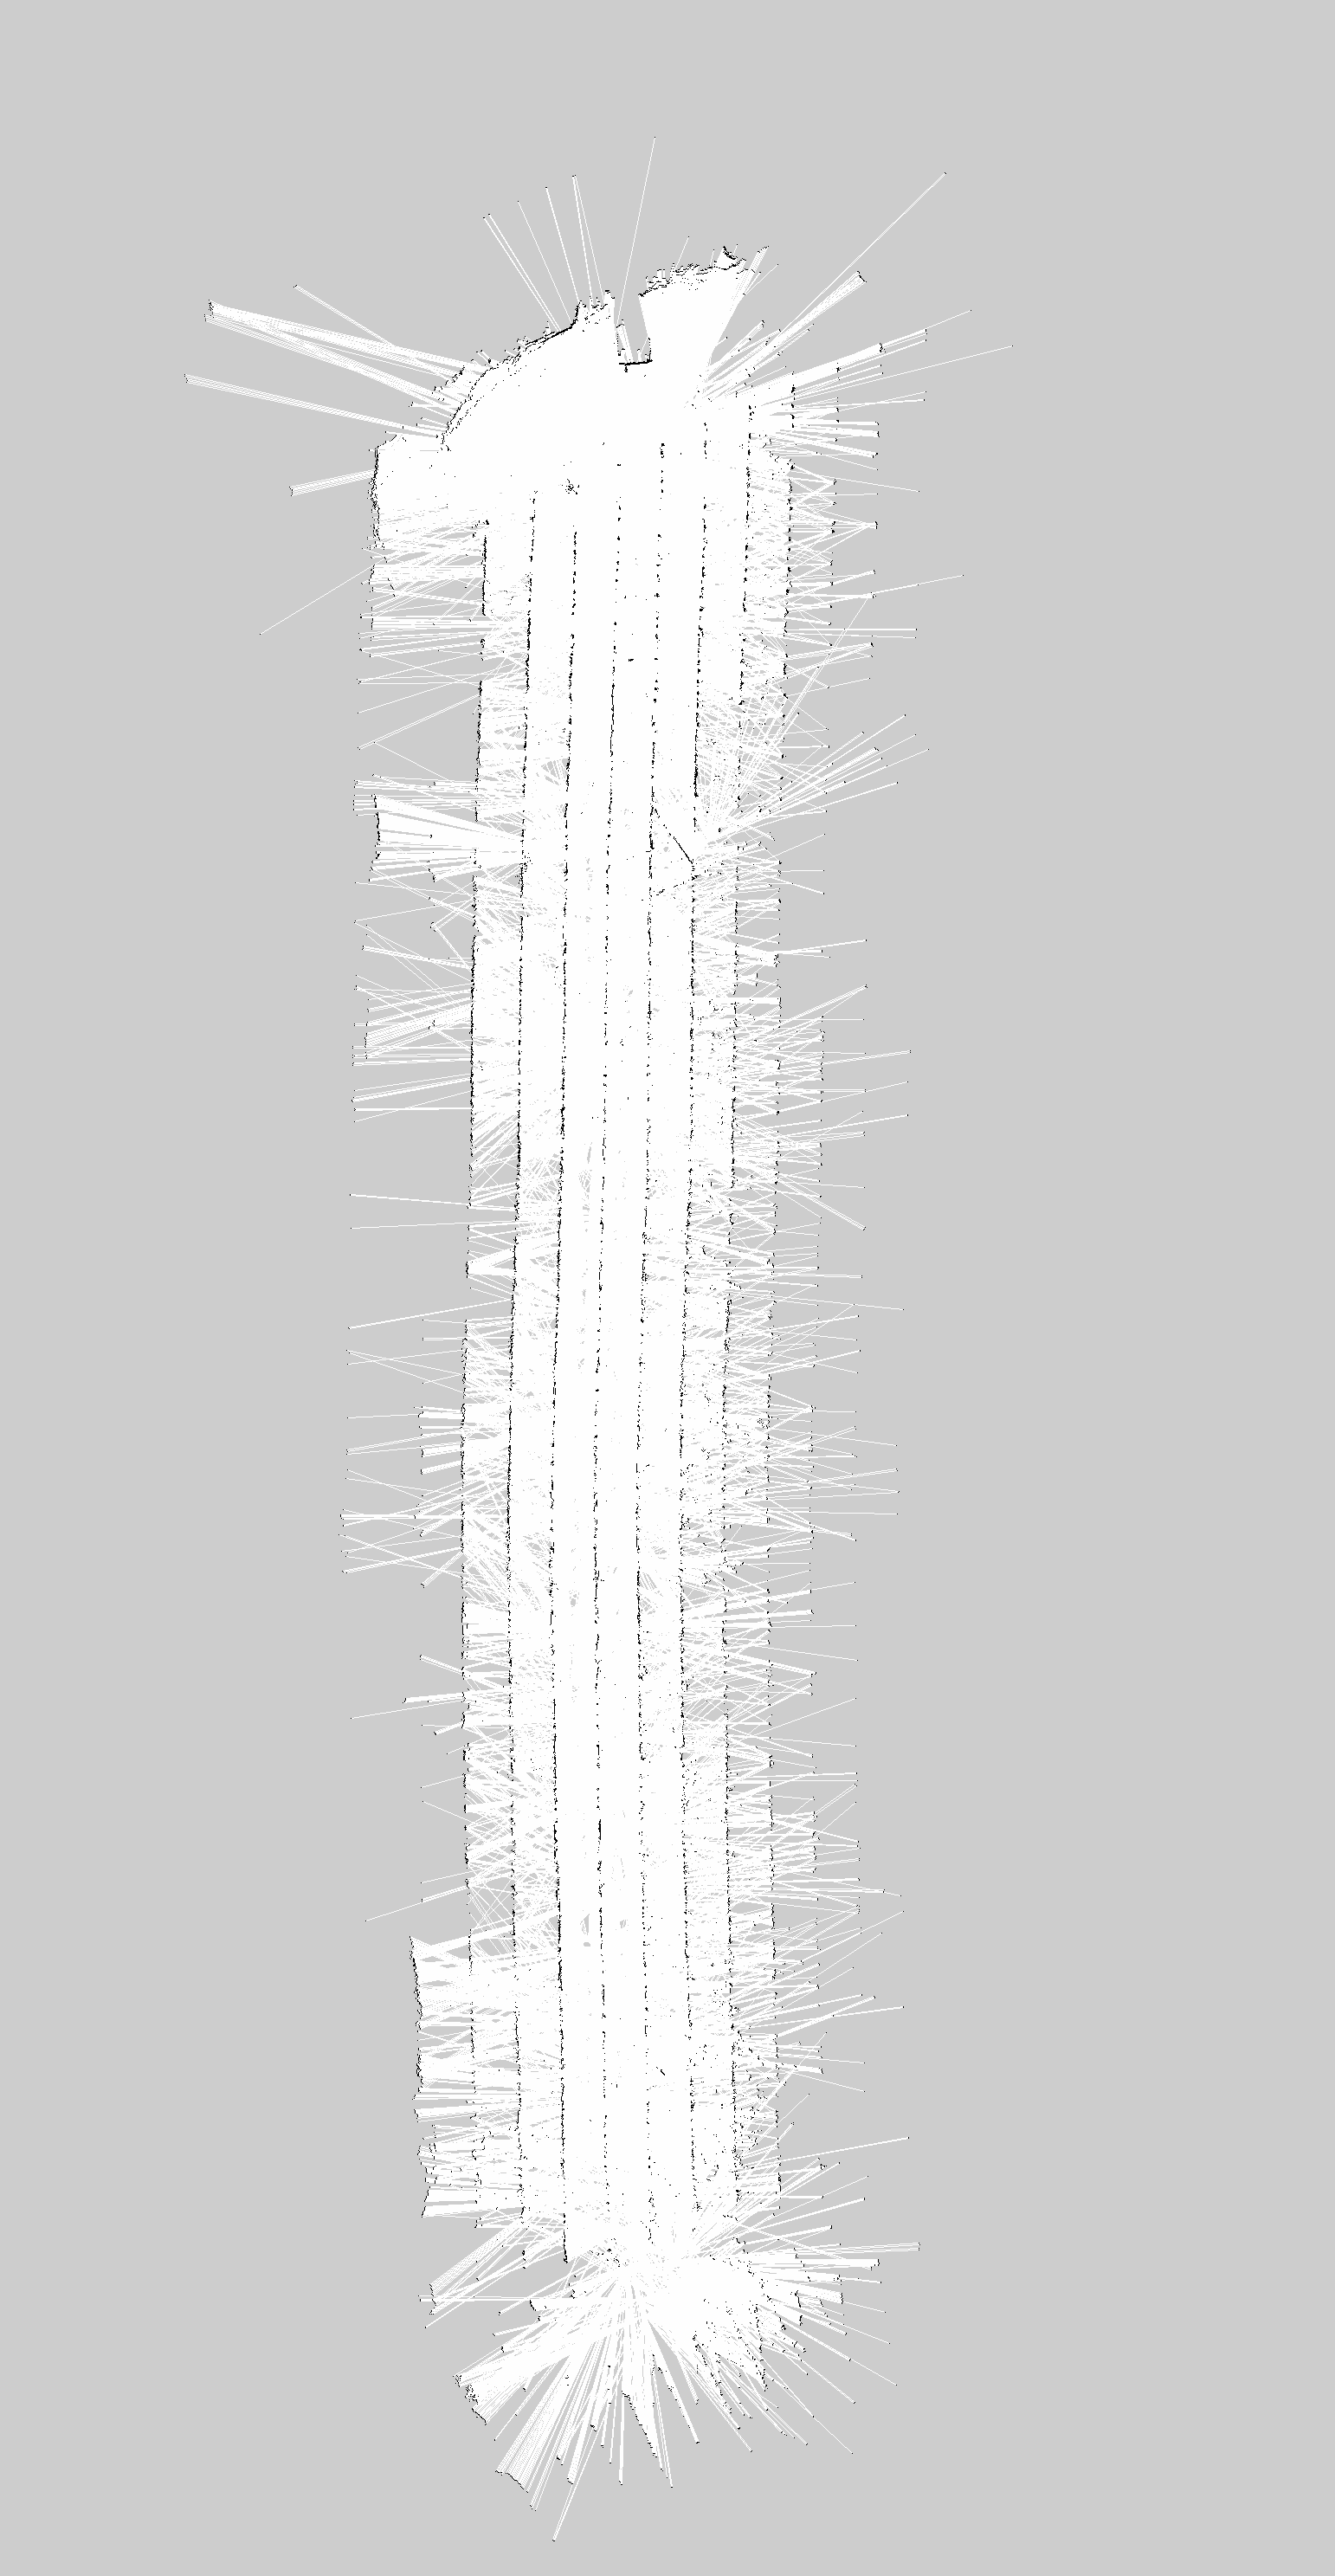
\includegraphics[width=1\textwidth]{Images/localization/map.png}
		\label{fig:vineyardMapIntera}}
	\end{minipage}
	\qquad
	\begin{minipage}[c]{.5\textwidth}
		\subfloat[]{%
		
\includegraphics[width=1\textwidth]{Images/localization/map_detail.png}
		\label{fig:vineyardMapDetail}}
	\end{minipage}
	\caption{\textit{Map of the Mas Llunes vineyard in Garriguella (ES), computed during the last integration week using Robot Localization and Gmapping. In \ref{fig:vineyardMapDetail}, a magnified detail.}}
	\label{fig:vineyardMap}
\end{figure}

\begin{figure}
	\centering
	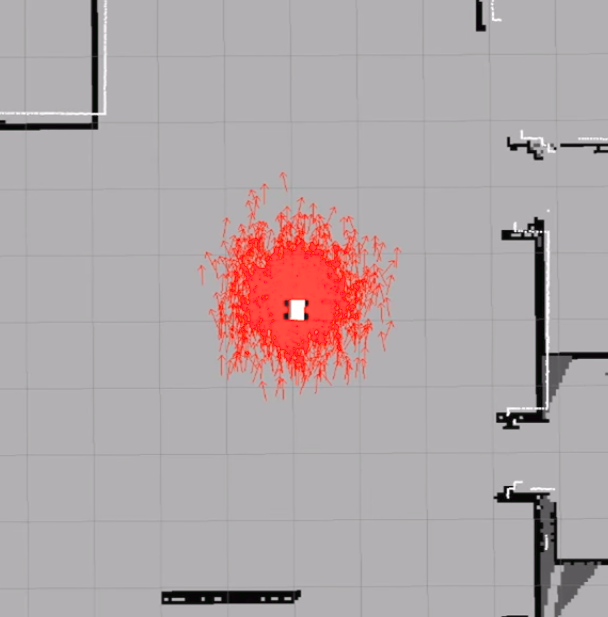
\includegraphics[width=0.5\textwidth]{Images/localization/amcl.png}
	\caption{\textit{Belief about the robot estimate using \ac{AMCL}, through a particles cloud where each particle represents a hypothesis about the real pose.}}
	\label{fig:amclAlgoritmo}
\end{figure}

\ac{AMCL} with laser scanners provides a very effective localization in feature-rich environments, like in typical indoor environments with very sharp corners and well defined obstacles, as the ones in Figure \ref{fig:amclAlgoritmo}.
However, as hinted at the beginning of this Section, a few tests were sufficient to show the weakness of this localization algorithm in our context, due to the high repetitiveness of the vineyard map. In Figure \ref{fig:vineyardMapDetail} you can see a magnified detail of the map of Mas Llunes vineyard, computed using Robot Localization as odometry system, and Gmapping for \ac{SLAM}; most of the obstacles detected by the frontal \ac{LIDAR} are the trunks of the trees, together with poles and high weeds.
 It's intuitive that if the map in which the robot moves presents a lot of repeated patterns, the \textit{survival of the fittest} paradigm that the \textit{sensor update} step of \ac{AMCL} should implement is not very effective. Moreover, note that the bumpiness of the terrain leads the plan that the \ac{LIDAR} scans to change significantly its orientation in time. So, for example, given a position in the map, the sensed obstacles over time in this location could be different portions of the same vine, then the shape is likely not to be constant.

\item[Row crossing problem] \hfill \\
The vineyard environment also presented another criticality, due to the average distance between the vines belonging to the same row; indeed, because of the height of the \ac{LIDAR} used for obstacles detection, the trunks of the plants are detected while the horizontal branches of the vines often are not.
If this situation occurs, the space between the trees is sensed as free of obstacles, even if the horizontal branches of the vines are an actual obstacle to the \ac{UGV}. The first attempt to solve this problem was to simply provide an higher inflation radius (see Section \ref{sec:motionPlanning}) to the obstacles, in order to fill the gaps between a plant and the adjacent ones. However, this naive solution couldn't find a trade-off to the extreme situations:
\begin{itemize}
	\item a too small inflation radius is not able to provide a solution to the problems \textit{i.e.} fill the gaps between adjacent trees
	\item an inflation radius large enough to fill the aforementioned gaps, makes the navigation almost impossible, because even a small obstacle among two rows (\textit{e.g.} some weed) completely occludes the path.
\end{itemize}

\end{description}

\subsection{Insertion of prohibition layer}\label{subsec:virtualFences}
Given the impossibility to solve the problem of row crossing with the standard inflation radius of the obstacle layer, we found a very effective solution that relies on the very simple global structure of the vineyard. Indeed, looking at the map in Figure \ref{fig:vineyardMapIntera}, it's easy to notice that the obstacles that cause the row crossing problem are of course aligned, and parallel to each other, so the idea was to implement a series of "virtual fences" corresponding to the vine rows. The implementation was possible thanks to a feature of \textit{costmap\_2d}, the package of \ac{ROS} responsible of the creation of the occupancy grid maps. Indeed, this package implements a \textbf{layered} costmap: this means that, for example, the global and local costmaps (see Section \ref{sec:motionPlanning}) live in two different layers, that are computed independently:
\begin{itemize}
	\item the global costmap is computed from the obstacles described in the occupancy grid map, possibly inflated of a chosen radius
	\item the local costmap is computed in a spacial window around the robot position, from the obstacles detected by the laser scans. The obstacles possibly are inflated of a chosen radius
\end{itemize}
Since an arbitrary number of custom layers can be added by implementing C++ base class \textit{costmap\_2d::Layer} of Move Base package, two additional layers were introduced, in order to include the virtual obstacles of the rows both in global and local costmap:
\begin{itemize}
	\item \textbf{Global prohibition layer:} this includes the virtual fences in the global costmap, and it's useful for the global planner to take them into account for the creation of the global navigation plan
	\item \textbf{Local prohibition layer:} this includes the virtual fences in the local costmap, and it's useful for the local planner to take them into account for the creation of the local navigation plan. This is required because otherwise the local planner might over-optimize the global plan and, however take advantages of the gap between the plants. This situation is comparable to an indoor planning problem in which a local planner detects an open door that was shut at mapping time: even if the global path doesn't take advantage of the door gap, the local planner might choose to traverse it if it reduces the motion execution cost.
\end{itemize}

\subsection{Switch to mapless navigation}
After several effort in Move Base parameter tuning, the role of  \ac{AMCL} in the poor performance in navigation tasks was clear. Since the map in navigation task is useful in terms of:
\begin{itemize}
	\item \textbf{global planning}: it provides a set of obstacles that helps the robot to optimize the global path in planning phase. See for example Figure \ref{fig:mapGlobalPlanner}: if no map was provided, the global plan would have been a straight line between the start and the goal states, and all the obstacle avoidance lies on local planner. This of course can lead to a performance degradation, because the knowledge of some obstacles in advance often brings to much more efficient global plans.
	\item \textbf{localization}: in order to provide an estimate of the robot pose in the environment (for example, through \ac{AMCL})
	\item \textbf{visualization}: to better contextualize the position of the robot for human users. 
\end{itemize}

Given the problems caused by \ac{AMCL}, we decided to switch to a \textbf{mapless} navigation configuration, because we were able to compensate all the advantages of the mapped navigation using other tools or methods:

\begin{itemize}
	\item \textbf{global planning}: as we already pointed out in Subsection \ref{subsec:virtualFences}, even if the vineyard environment is strongly unstructured at fine-grained level (for the reasons explained at the beginning of this Section), it has a fixed and very simple global structure given by the parallel vine rows, as you can see in vineyard maps (Figure \ref{fig:vineyardMap}). Thus, the inclusion of the virtual fences layers only in the global costmap is a simple, but very effective approximation of the vineyard global map.
	\item \textbf{localization}: in both our field test locations (Casciana Terme (IT) and Garriguella (ES)), we could rely on high-precision RTK GPS \parencite{rtk} as input for the \ac{UGV} odometry system. Even if RTK correction worldwide coverage is not guaranteed, several companies exist that provide this service. For example, see Figure \ref{fig:rtkItaly} for a map of RTK stations provided in Italy by the sole SmartNet Italy\footnote{\url{http://it.smartnet-eu.com/}}
company. Moreover, since our navigation tasks are executed outdoor, the assumption of an high-precision GPS system is reasonable and we only need to specify the virtual fences positions through the GPS coordinates of their endpoints to navigate the virtual fences costmap layer.
	\item \textbf{visualization}: in this configuration our \ac{UGV} is always geolocalized; so, we can contextualize the robot position for human users by overlaying to the robot position the corresponding satellite images, using for example the \textit{AerialMapDisplay} plugin for RViZ.
\end{itemize}
Since we were able to compensate for all the advantages of the navigation with a map, we decided to switch to a mapless configuration, at the cost of adding the assumption of high-precision GPS and geolocalized virtual fences at disposal. Note that, in this configuration, the \textit{localization} task is not relevant anymore since there is not an actual map to localize into; then the \textit{tf} transform from \textit{map} to \textit{odom} is reduced to the identity transformation.


\begin{figure}
	\centering
	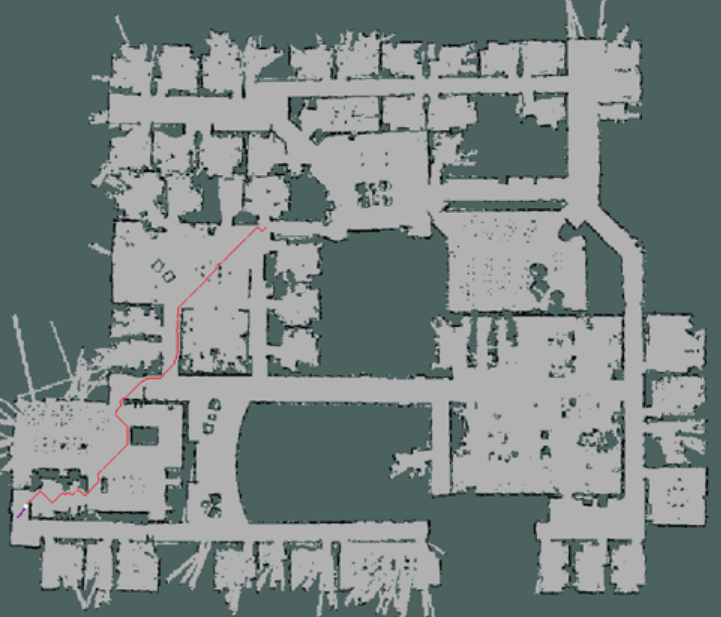
\includegraphics[width=0.7\textwidth]{Images/localization/map_global_planner.png}
	\caption{\textit{Example of global plan that takes into account the map obstacles.}}
	\label{fig:mapGlobalPlanner}
\end{figure}

\begin{figure}
	\centering
	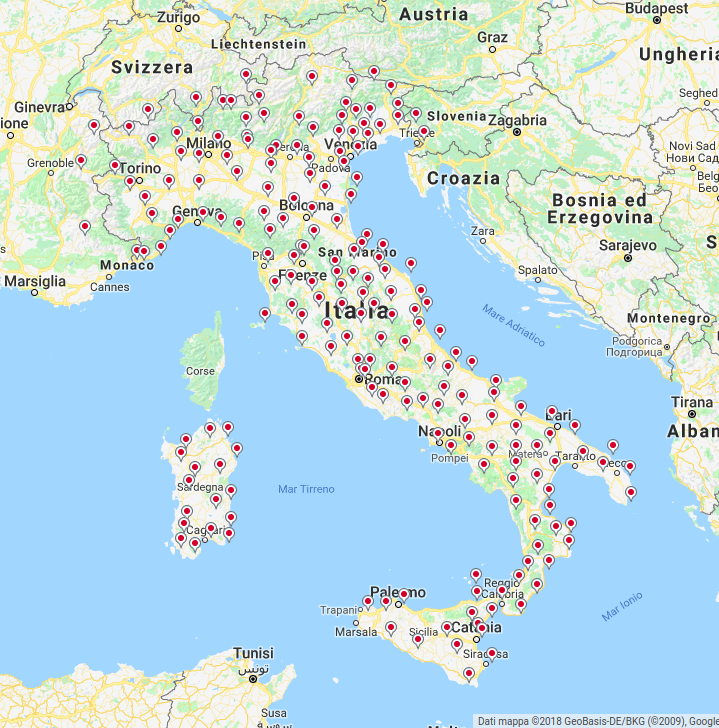
\includegraphics[width=0.7\textwidth]{Images/localization/rtkItaly.png}
	\caption{\textit{RTK stations provided by SmartNet Italy.}}
	\label{fig:rtkItaly}
\end{figure}

\subsection{Switch to Timed Elastic Band as local planner}
Also the standard local planner of Move Base, a \ac{ROS} implementation of Dynamic Window Approach \parencite{dwa}, showed some weak points in the vineyard context. In Figure \ref{fig:localCostmap} you can see an example of local costmap, computed during an autonomous navigation tasks in Garriguella: the virtual fences are highlighted in blue, the obstacles detected by the frontal \ac{LIDAR} in pink, and the inflation layer in light blue. Since the detected obstacles are mainly tree trunks, they are detected as small, non continuous obstacles. The inflation of such obstacles leads to a jagged border of the resulting obstacle cells set. If, for example, the detected obstacle was a straight wall, the resulting obstacle layer would have been much more straight and sharp. Dynamic Window Approach had some problems to deal with such a large amount of dead ends, and often got stuck in the obstacle contours (see Figure \ref{fig:dwaStuck}). Thus, we switched to another \textit{off-the-shelf} local planner, compatible with the Move Base local planner interface: an implementation for \ac{ROS} of the \textit{Timed Elastic Band} algorithm \parencite{teb}. This algorithm, at the cost of an higher computational load, provided much more robust navigation.

\begin{figure}
	\centering
	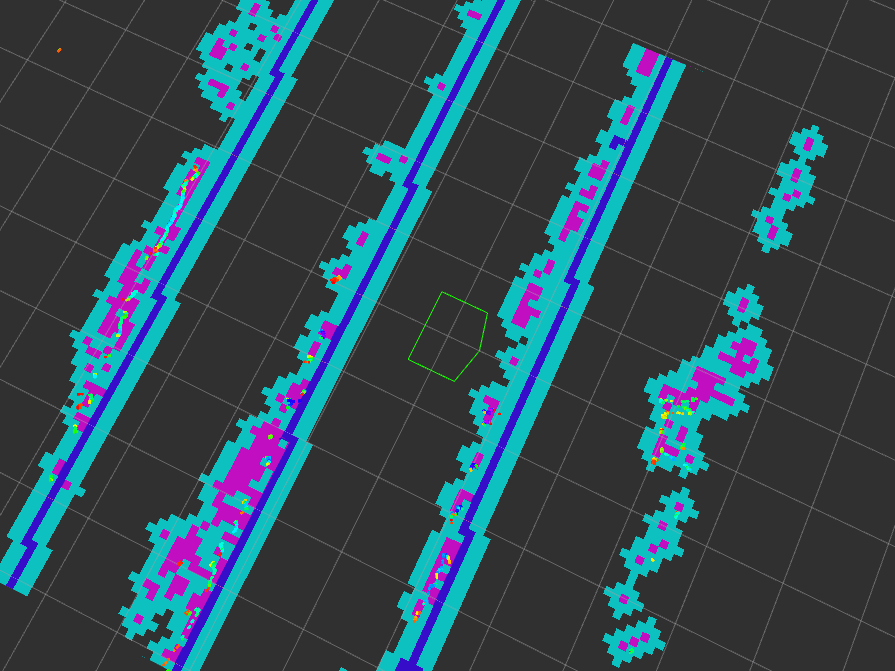
\includegraphics[width=0.7\textwidth]{Images/localization/localCostmap_highlighted.png}
	\caption{\textit{Example of local costmap, in the final configuration: you can distinguish the virtual fences (blue), the obstacles detected by the \ac{LIDAR} (pink), and the inflation layer (light blue). The green polygon represents the robot footprint.}}
	\label{fig:localCostmap}
\end{figure}

\begin{figure}
	\centering
	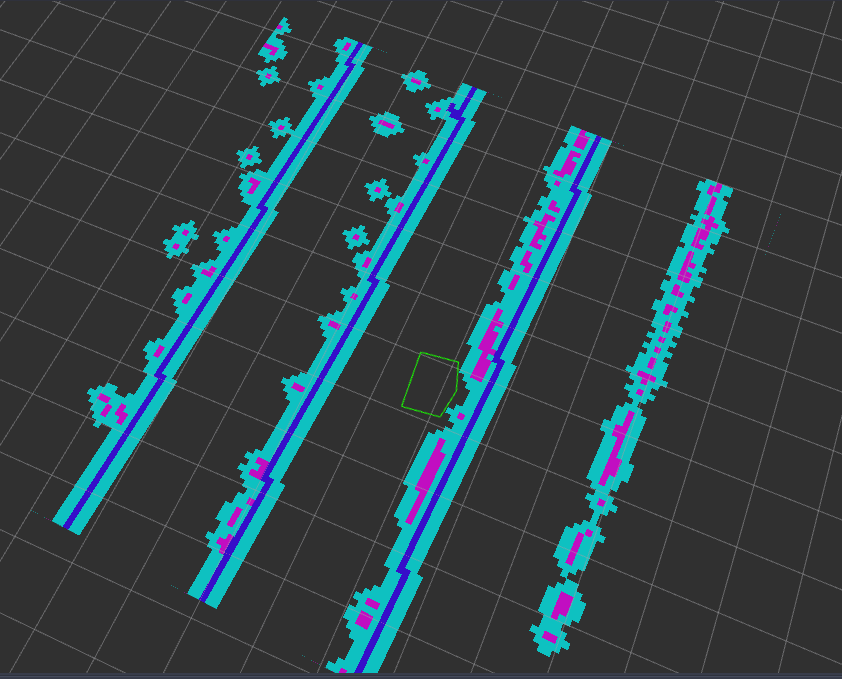
\includegraphics[width=0.7\textwidth]{Images/localization/localCostmap_stuck.png}
	\caption{\textit{Example of local plan computed by DWA that get stuck in the jagged border of the obstacles.}}
	\label{fig:dwaStuck}
\end{figure}

\subsection{AMCL as input to sensor fusion}
In the late phases of the \ac{GRAPE} project, some efforts were made to, however, take advantage in some way of \ac{AMCL} algorithm potential. In particular, the alignment with the sensed laser scans could lead to the following benefits:
\begin{itemize}
	\item better estimate of the robot orientation 
	\item compensate for the measurement errors of the GPS, since the virtual fences are specified through GPS coordinates of the endpoints
\end{itemize}

We already highlighted the strong drawbacks due to using \ac{AMCL} as localization algorithm, so the attempt was to disable its publication of the \textit{tf} transform from \textit{map} to \textit{odom}, and fuse its estimated pose together with the other sensor inputs in the Robot Localization node. In this way the weaknesses of \ac{AMCL} alone are likely to be compensated from the other sensors' estimates. If this configuration had resulted effective, switching back to a navigation with map would have been a reasonable choice. Unfortunately, due to the lack of time (final review of \ac{GRAPE} project was held in March, 21$^{st}$, 2018), this configuration was not sufficiently tested. 

However, the tests that were performed were sufficient to highlight some difficulties in the coexistence of GPS and \ac{AMCL} as input sources in the Robot Localization nodes, probably for these reasons:
\begin{itemize}
	\item Low publishing rate of both \ac{AMCL} and GPS (\textasciitilde 1 second)
	\item Pose estimates always discordant between them, maybe for some misconfiguration or bias of GPS module
\end{itemize}
For this reason, the output pose of Robot Localization suffered of constant jumps between the estimate of GPS and the one of \ac{AMCL}, instead of keeping both of them into account. In Figure \ref{fig:amclRobotLocalization} an example is provided of discordance between the estimate from \ac{AMCL} (represented by the particles position) and the one from GPS (corresponding in the figure to the actual estimated pose).


\begin{figure}
	\centering
	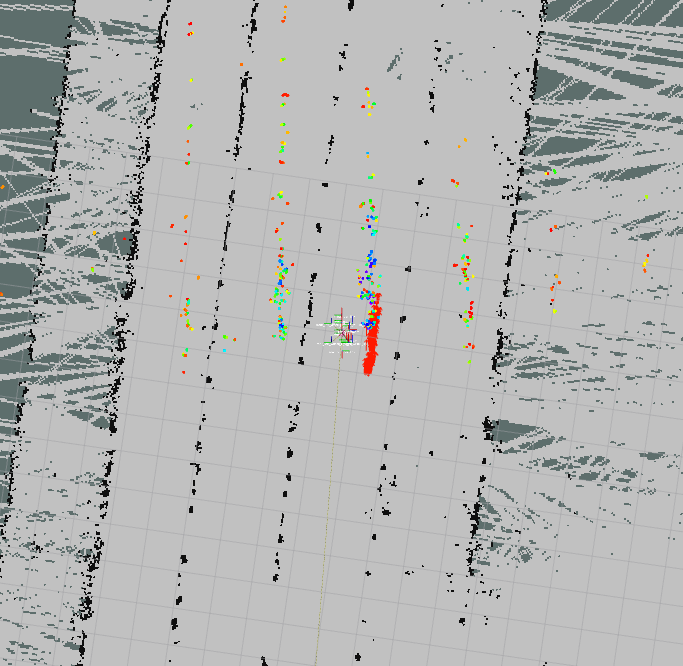
\includegraphics[width=0.7\textwidth]{Images/localization/amcl_robot_localization.png}
	\caption{\textit{Example of conflict between the pose estimated from \ac{AMCL} (displayed by the particles positions), and the final Robot Localization output (displayed by tf frames).}}
	\label{fig:amclRobotLocalization}
\end{figure}




